A non-anthropomorphic robotic platform was created to no influence participants' perception. The robotic platform is holonomic and it was built using Odroid U3, Arduino Due, and 3 metal gear motors with 64 CPR encoders and omniwheels. The platform could be observed in Figure~\ref{fig:Robot}. The Arduino Due is in charge to be the interface between the hardware (e.g. motors) and Odroid, which host all the Emotion Enrichment System.

\begin{figure}[t]
\centering%
\subfigure {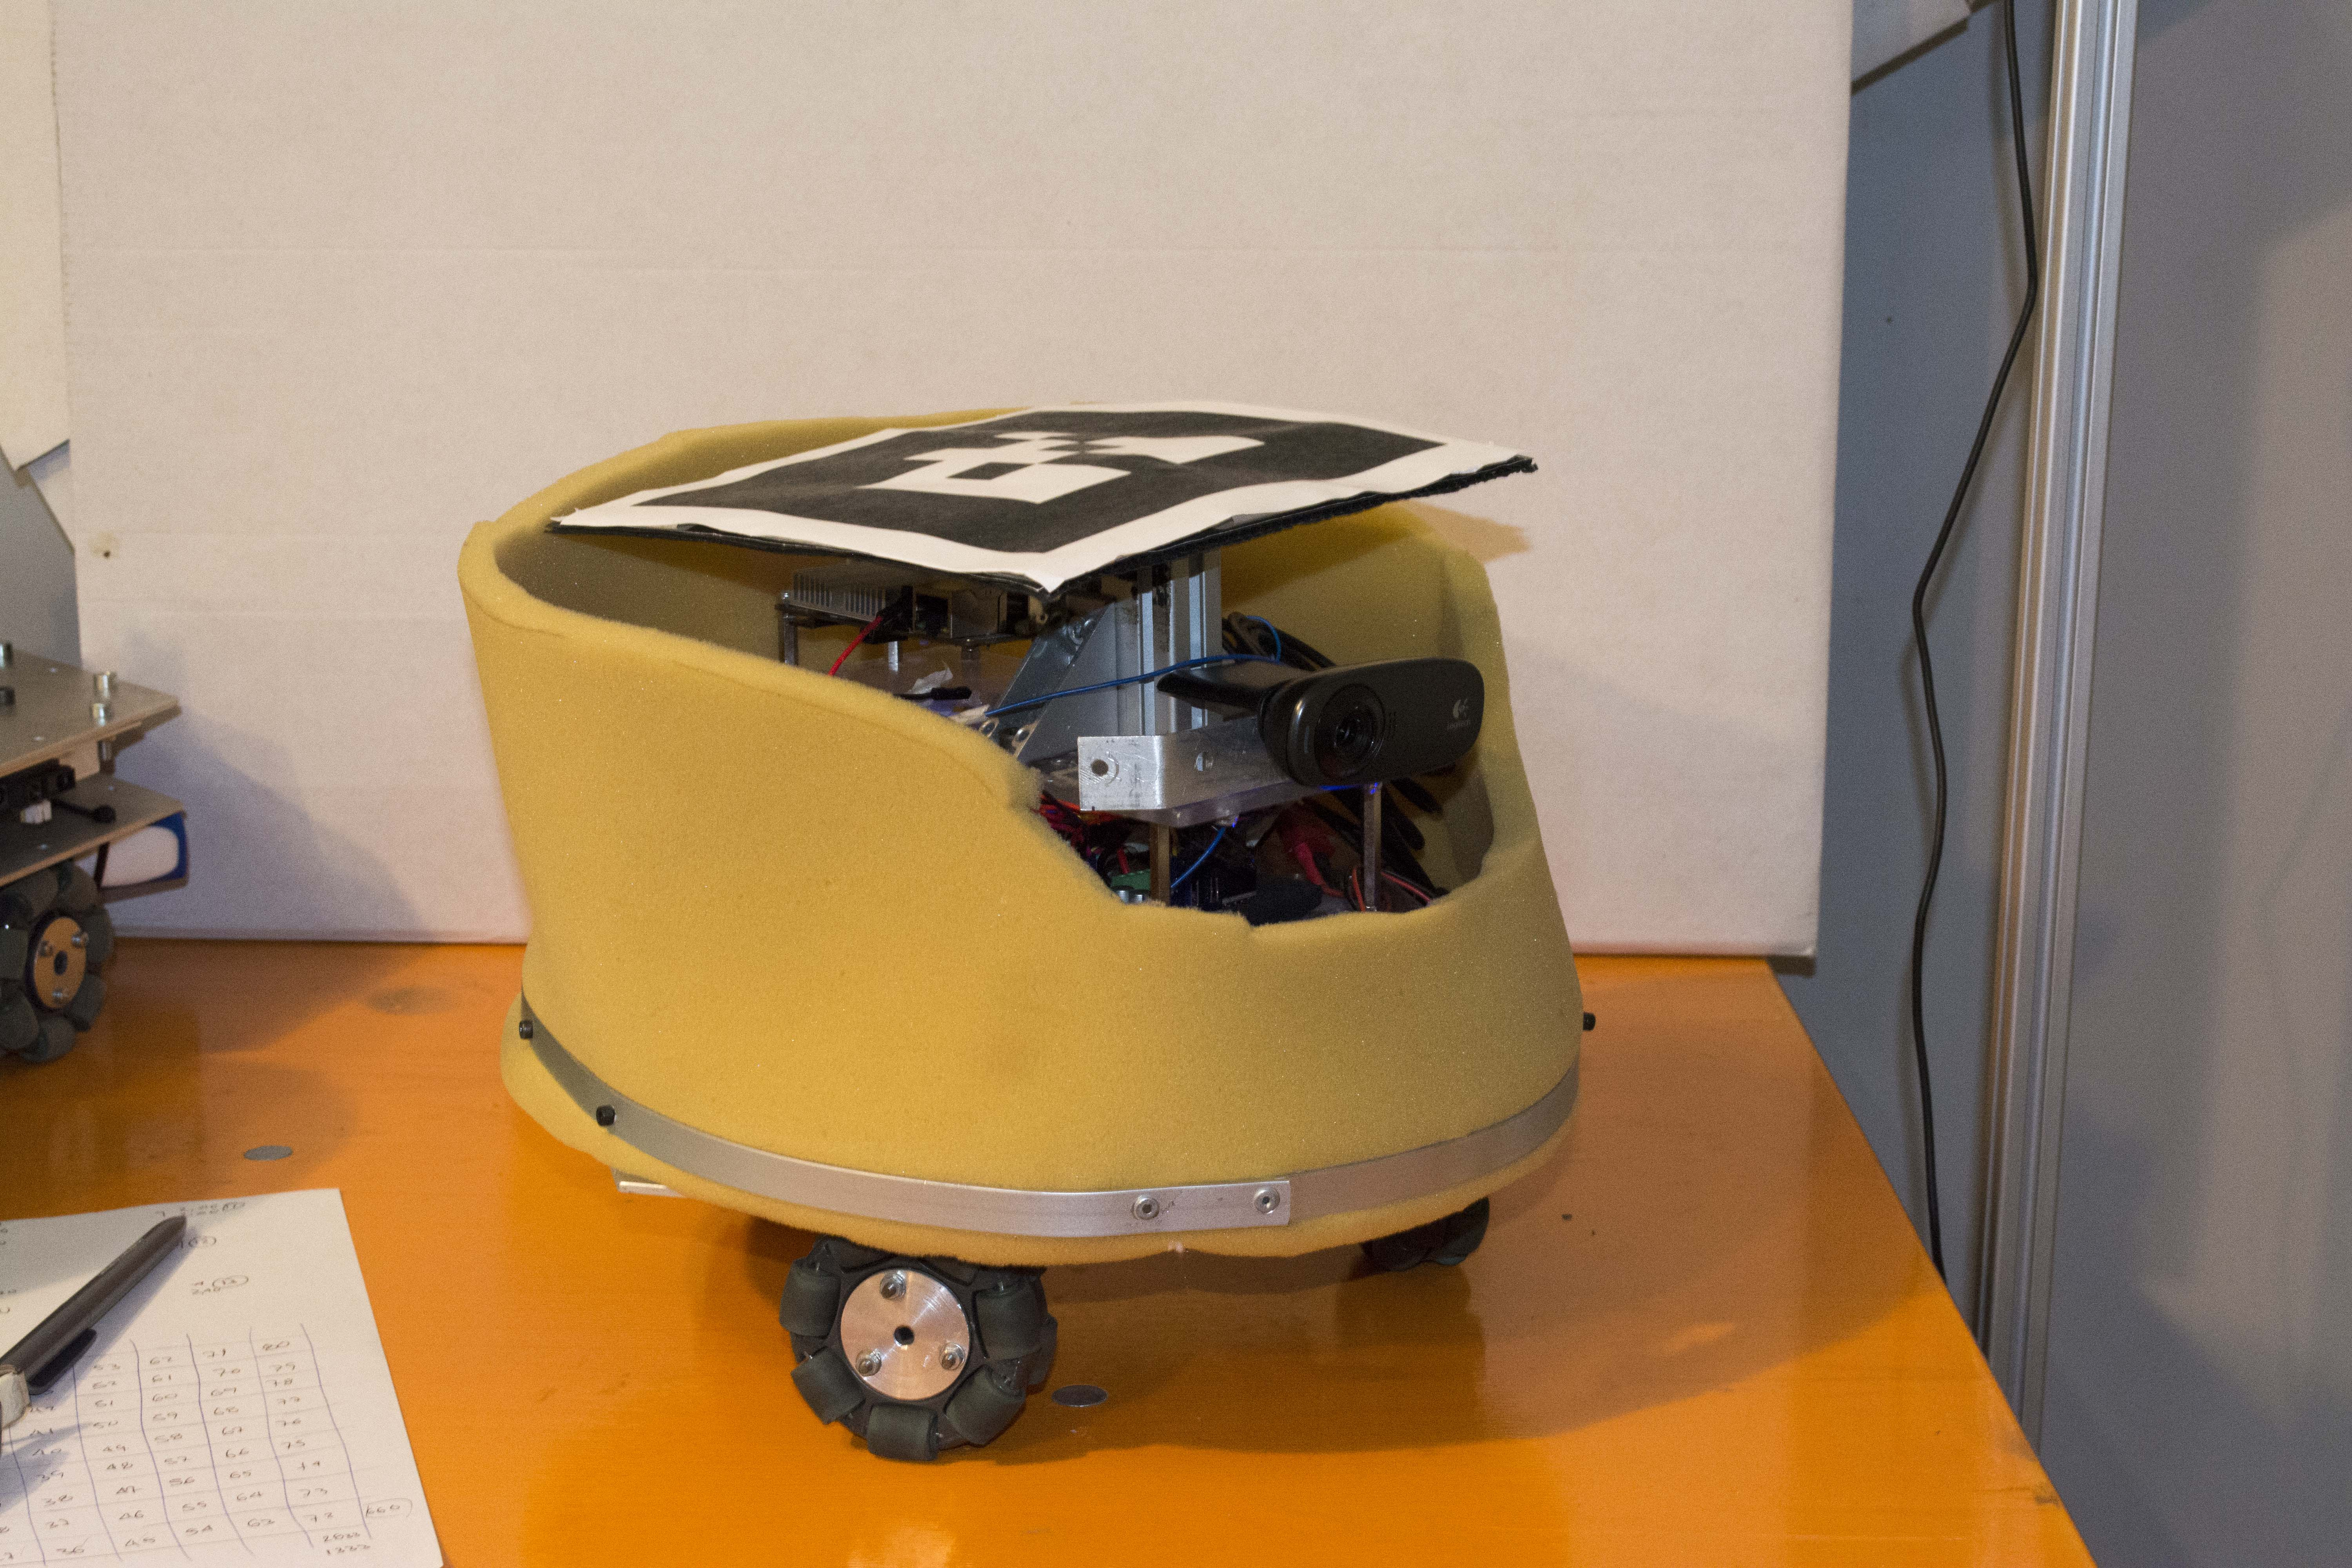
\includegraphics[height=3cm]{./Images/DSC_0447.JPG}}
\hspace{2mm}
\subfigure{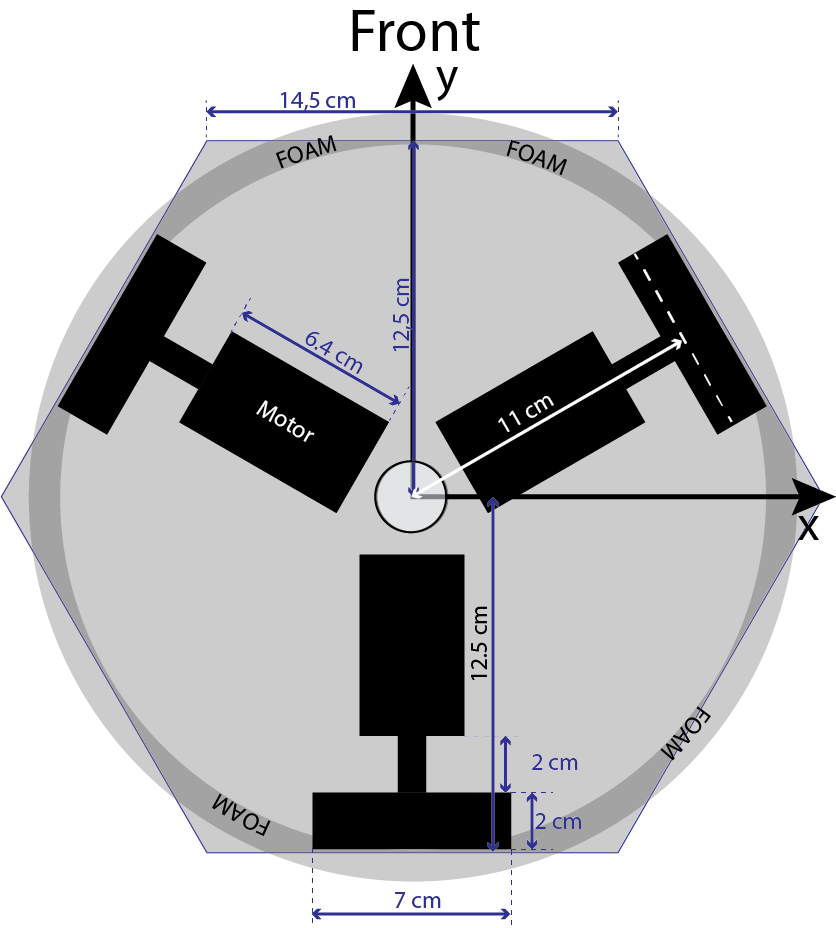
\includegraphics[height=3cm]{./Images/TriskarThird.png}}
\caption{Platform used in the case study (left), and holonomics's blue prints (right). The arrows represent robot's frame of reference.
\label{fig:Robot}}
\end{figure}

An Emotional Enrichment System was designed and implemented to automatize the process of emotion expression~\cite{Angel2017}. It modifies actions' parameters and adds additional actions to create the illusion of emotion expression in a robot. To achieve this, the system receives two messages. One message describes actions and the order in which they should be executed. These actions could be executed in parallel, sequentially or a combination of both. This kind of description enables the possibility to communicate several actions in one message. The other message informs the system with the desire emotion and its intensity. These two messages could arrive asynchronously and without any particular order. Every time a message is received, the system updates the robot movements to convey the desire emotion in the specific action.